\documentclass[12pt,a4paper,twoside]{book}
\usepackage{graphicx}
\usepackage{setspace}	%double spacing for text, single for captions, footnotes, etc.
%\usepackage{hypernat} 	%substitut de cite que permet fer hyperlinks
\usepackage{natbib}		% substituye a 'hypernat' que funciona en Windows.
\usepackage[spanish]{babel}
\usepackage[utf8]{inputenc}
\usepackage{color}
\usepackage{hhline} 		% extended styles for tables
\usepackage{multirow}
\usepackage{subfigure}
\usepackage{acronym}
\usepackage{hyperref}
\usepackage{amsmath,amsmath,amssymb} 
\usepackage{fancyhdr}
\usepackage{epsfig, amsmath}
\usepackage{algorithm}
\usepackage{algorithmic}
\usepackage{url}
\usepackage{listings}

% general settings
\hypersetup{
	linktocpage=true,
	colorlinks=true,
	linkcolor=blue,
	citecolor=blue,
}
\definecolor{Hgray}{gray}{0.6}

\newenvironment{definition}[1][Definition]{\begin{trivlist}
\item[\hskip \labelsep {\bfseries #1}]}{\end{trivlist}}

\setlength{\topmargin}{0cm}
\setlength{\textheight}{23cm}
\setlength{\textwidth}{17cm}
\setlength{\oddsidemargin}{0cm}
\setlength{\evensidemargin}{0cm}
\setlength{\headheight}{1cm}

% indica que las 'sub-sub-sections' sean numeradas y aparezcan en el indice
\setcounter{secnumdepth}{3}
\setcounter{tocdepth}{2}

% settings for code
\renewcommand{\algorithmicrequire}{\textbf{Entrada: }}
\renewcommand{\algorithmicensure}{\textbf{Salida: }}

% estilos de codigo
\definecolor{codegreen}{rgb}{0.07, 0.4, 0.27}
\definecolor{codegray}{rgb}{0.5,0.5,0.5}
\definecolor{codepurple}{rgb}{0.5,0.08,0.3}%{0.5,0.8,0.3}
\definecolor{codeblue}{rgb}{0.06,0.21,1.0}
\definecolor{backcolour}{rgb}{0.97,0.97,0.97}

\lstdefinestyle{mystyle}{
    language=Python,
    texcl=true,
    backgroundcolor=\color{backcolour},   
    commentstyle=\color{codegreen},
    keywordstyle=\color{codepurple},%{magenta},
    numberstyle=\tiny\color{codegray},
    stringstyle=\color{codeblue},
    basicstyle=\scriptsize\sffamily,%\bfseries,
    breakatwhitespace=false,         
    breaklines=true,                 
    captionpos=b,                    
    keepspaces=true,                 
    numbers=left,                    
    numbersep=5pt,                  
    showspaces=false,                
    showstringspaces=false,
    showtabs=false,                  
    tabsize=2
}

\lstset{style=mystyle}%, inputencoding=utf8/latin1}

%%%%%%%%%%%%
% DOCUMENT %
%%%%%%%%%%%%
\begin{document}

% portada
\newpage
\thispagestyle{empty}

\baselineskip 2em

%\vspace*{1cm}

\centerline{
\includegraphics[width=0.6\textwidth]{images/UOC-logo}}
\begin{center}
\textsc{Universitat Oberta de Catalunya (UOC) \\
 Máster Universitario en Ciencia de Datos (\textit{Data Science})\\}

%\centerline {\pic{UOC}{4cm}}

\vspace*{1.5cm}

\textsc{\Large TRABAJO FINAL DE MÁSTER}

\vspace*{0.5cm}

\textsc{\large Área: Big Data Analytics}


%\textbf{\Huge VirtualTechLab Model: }

\vspace*{2.0cm}

\textbf{\Large Análisis predictivo del comportamiento de los clientes \\
en sus interacciones con la empresa}

\vspace{2.5cm}
\baselineskip 1em

\baselineskip 2em
-----------------------------------------------------------------------------\\
Autor:      Diego Contreras Jiménez\\
Tutor:      Jordi Nin Guerrero\\
Profesor:   Jordi Casas Roma\\
-----------------------------------------------------------------------------\\
\vspace*{1.5cm}
Barcelona, \today

\end{center}

\newpage
\pagestyle{empty}
\hfill

\newpage

% abstract
\pagenumbering{roman} 
\setcounter{page}{1} 
\pagestyle{plain}

%%%%%%%%%%%%%%%%
%%% CREDITOS %%%
%%%%%%%%%%%%%%%%
\chapter*{Copyright}

\vspace{1cm}

\begin{figure}[ht]
    \centering
	
\includegraphics[scale=1]{images/license.png}
\end{figure}
\\
Esta obra está sujeta a una licencia de Reconocimiento -  NoComercial - SinObraDerivada
\\
\href{https://creativecommons.org/licenses/by-nc-nd/3.0/es/}{3.0 España de CreativeCommons}.
\\
Esta obra está sujeta a una licencia de Reconocimiento-NoComercial- SinObraDerivada 3.0 España de Creative Commons
\\
\\
\\
Copyright © 2019 Diego Contreras Jiménez
\\
\\
Reservados todos los derechos. Está prohibida la reproducción total o parcial de esta obra por cualquier medio o procedimiento, comprendidos la impresión, la reprografía, el microfilme, el tratamiento informático o cualquier otro sistema, así como la distribución de ejemplares mediante alquiler y préstamo, sin la autorización escrita del autor o de los límites que autorice la Ley de Propiedad Intelectual.

%%%%%%%%%%%%%
%%% FICHA %%%
%%%%%%%%%%%%%
\chapter*{FICHA DEL TRABAJO FINAL}

\begin{table}[ht]
	\centering{}
	\renewcommand{\arraystretch}{2}

	\begin{tabular}{r | l}
		\hline
		Título del trabajo: & Análisis predictivo del comportamiento de los clientes \\ & en sus interacciones con la empresa \\
		\hline
        Nombre del autor: & Diego Contreras Jiménez\\
		\hline
        Nombre del colaborador docente: & Jordi Nin Guerrero\\
		\hline
        Nombre del PRA: & Jordi Casas Roma\\
		\hline
        Fecha de entrega: & 06/2019\\
		\hline
        Titulación o programa: & Máster universitario de Ciencia de datos\\
		\hline
        Área del Trabajo Final: & Big Data Analytics\\
		\hline
        Idioma del trabajo: & Español\\
		\hline
        Palabras clave & Predictive analytics \\ & User interactions \\ & Customer experience\\
		\hline
	\end{tabular}
\end{table}

%%%%%%%%%%%%%%%%%%%
%%% DEDICATORIA %%%
%%%%%%%%%%%%%%%%%%%
\chapter*{Cita}

``Information is the oil of the 21st century, and analytics is the combustion engine" 

(Peter Sondergaard, Senior VP, Gartner).

%%%%%%%%%%%%%%%%%%%
%%% Agradecimientos %%%
%%%%%%%%%%%%%%%%%%%
\chapter*{Agradecimientos}

Gracias a mi pareja Erika, que ha estado siempre apoyándome y ayudándome en todo lo posible para que pudiera dedicarme a la realización de este trabajo y a la culminación del mismo.
\\
Tampoco puedo dejar de agradecer a mi tutor de máster Jordi Nin Guerrero que, con su esfuerzo y dedicación, sus conocimientos y certera dirección hicieron posible la realización de este trabajo.
\\
\\
A todos, mi más sincera gratitud.
\\
El autor


%%%%%%%%%%%%%%%%
%%% RESUMEN  %%%
%%%%%%%%%%%%%%%%
\chapter*{Abstract}
\addcontentsline{toc}{chapter}{Abstract}

\onehalfspacing

Customers communicate with companies through several ways (e.g., phone, web, mobile applications, social networks, e-mail...). The purpose of these interactions can be for different reasons, for example:
\begin{itemize}
  \item Obtaining information on products and prices.
  \item Consulting invoices.
  \item Making claims for any problem with their service.
  \item Contracting new products or services.
  \item Modifying any terms of existing contracts.
  \item Terminating the contract itself.
\end{itemize}

Companies usually have CRM systems which manage interactions with existing and potential customers. An important feature of these systems is that they allow information to be collected from the different channels.

In the case of large companies with millions of customers, processing all this data can be very complex and slow, but there are massive processing technologies such as parallel computing that allow to reduce time considerably.

The log of user interactions can be analyzed to understand their preferences and needs, so companies can improve business relationships with their customers and therefore, provide a better customer experience.

Artificial Intelligence and Machine Learning algorithms can be used to influence business decision making. For example, predictive analytics can lead to increase cross-selling and customer retention. In addition, all these improvements could have an impact on the reduction of operating costs derived from the impact of telephone calls to the call center. 

\vspace{1.5cm}

\textbf{Keywords}: Predictive analytics, User interactions, Customer experience 

\chapter*{Resumen}
\addcontentsline{toc}{chapter}{Resumen}

\onehalfspacing

Los clientes interactúan con las empresas a través de diversas formas de comunicación (e.g., teléfono, web, aplicaciones móviles, redes sociales, e-mail...). La finalidad de estas comunicaciones puede ser por distintos motivos, como por ejemplo: 

\begin{itemize}
  \item Obtener información de productos y precios.
  \item Consultar la facturación.
  \item Hacer reclamaciones por cualquier problema con su servicio.
  \item Contratar nuevos productos o servicios.
  \item Modificar cualquier condición de los contratos existentes.
  \item Dar de baja el propio contrato.
\end{itemize}

Las empresas suelen disponer de un sistema CRM en donde se gestionan las interacciones con los clientes, tanto los propios como los potenciales. Una funcionalidad importante de estos sistemas es que permiten recopilar información de los distintos canales. 

En el caso de las grandes empresas que cuentan con millones de clientes el procesamiento de todos estos datos puede ser muy complejo y lento, pero existen tecnologías de procesado masivo como la computación paralela que permiten reducir el tiempo considerablemente. 

Todo este historial de interacciones con los usuarios puede ser analizado posteriormente para comprender sus preferencias y necesidades, de modo que las empresas pueden mejorar las relaciones comerciales con sus clientes y por lo tanto ofrecer una mejor experiencia del cliente. 

Así pues, se puede hacer uso de algoritmos de Inteligencia Artificial y Machine Learning para influir en la toma de decisiones de la empresa. Por ejemplo, este análisis predictivo puede provocar un aumento de las ventas cruzadas y de la retención de clientes. Además, todas estas mejoras podrían repercutir en la reducción de los costes operativos derivados del impacto de las llamadas telefónicas al centro de llamadas.

\vspace{1.5cm}

\textbf{Palabras clave}: Analítica predictiva, interacciones de usuario, experiencia de usuario
\newpage

\pagestyle{fancy}
\renewcommand{\chaptermark}[1]{ \markboth{#1}{}}
\renewcommand{\sectionmark}[1]{\markright{ \thesection.\ #1}}
\lhead[\fancyplain{}{\bfseries\thepage}]{\fancyplain{}{\bfseries\rightmark}}
\rhead[\fancyplain{}{\bfseries\leftmark}]{\fancyplain{}{\bfseries\thepage}}
\cfoot{}

% indice
\cleardoublepage
\phantomsection
\addcontentsline{toc}{chapter}{Índice}
\tableofcontents

% listado de figuras
\cleardoublepage
\phantomsection
\addcontentsline{lof}{chapter}{Listado de Figuras}
\listoffigures

% listado de tablas
%\cleardoublepage
%\phantomsection
%\addcontentsline{lot}{chapter}{Listado de Tablas}
%\listoftables

% listado de codigo
\cleardoublepage
\phantomsection
\addcontentsline{lol}{chapter}{Listado de Código}
\lstlistoflistings

\thispagestyle{empty}

\pagenumbering{arabic}

\pagestyle{fancy}
\renewcommand{\chaptermark}[1]{ \markboth{#1}{}}
\renewcommand{\sectionmark}[1]{\markright{ \thesection.\ #1}}
\lhead[\fancyplain{}{\bfseries\thepage}]{\fancyplain{}{\bfseries\rightmark}}
\rhead[\fancyplain{}{\bfseries\leftmark}]{\fancyplain{}{\bfseries\thepage}}
\cfoot{}

\onehalfspacing

% capitulos del documento
\chapter{Introducción}
\label{chapter:introduccion}

%%% SECTION
\section{Título}

Análisis predictivo del comportamiento de los clientes en sus interacciones con la empresa.
 
 
%%% SECTION
\section{Palabras clave}

\begin{itemize}
    \item Predictive analytics  
    \item User interactions 
    \item Customer experience 
\end{itemize}

%%% SECTION
\section{Resumen de la propuesta}

Los clientes interactúan con las empresas a través de diversas formas de comunicación (teléfono, web, aplicaciones móviles, redes sociales, e-mails...). La finalidad de estas comunicaciones puede ser por distintos motivos, como por ejemplo: 

\begin{itemize}
  \item Obtener información de productos y precios.
  \item Consultar la facturación.
  \item Hacer reclamaciones por cualquier problema con su servicio.
  \item Contratar nuevos productos o servicios.
  \item Modificar cualquier condición de los contratos existentes.
  \item Dar de baja el propio contrato.
\end{itemize}

Las empresas suelen disponer de un sistema CRM en donde se gestionan las interacciones con los clientes, tanto los propios como los potenciales. 

Una funcionalidad importante de estos sistemas, es que permiten recopilar información de los distintos canales. 

En el caso de las grandes empresas que cuentan con millones de clientes el procesamiento de todos estos datos puede ser muy complejo y lento, pero existen tecnologías de procesado masivo como la computación paralela que permiten reducir el tiempo considerablemente. 

Todo este historial de interacciones con los usuarios puede ser analizado posteriormente para comprender sus preferencias y necesidades, de modo que las empresas pueden mejorar las relaciones comerciales con sus clientes y por lo tanto ofrecer una mejor experiencia del cliente. 

Así pues, se puede hacer uso de algoritmos de Inteligencia Artificial y \textit{``Machine Learning"} para influir en la toma de decisiones de la empresa. Por ejemplo, este análisis predictivo puede provocar un aumento de las ventas cruzadas y de la retención de clientes. Además, todas estas mejoras podrían repercutir en la reducción de los costes operativos derivados del impacto de las llamadas telefónicas al centro de llamadas. 


%%% SECTION
\section{Justificación}

Existen diversos canales para la comunicación entre las empresas y sus clientes, como pueden ser el teléfono, la web, las aplicaciones móviles, las redes sociales o los correos electrónicos. Aunque todos estos canales no ofrecen las mismas funcionalidades, muchas tareas se pueden realizar desde varios canales.

En la actualidad muchas empresas están enfocando sus esfuerzos a usar cada vez más la estrategia de contenidos ``omnichannel", que pretende mejorar la experiencia de usuario. El objetivo de esta estrategia es orquestar los múltiples canales de comunicación para que se integren y cooperen entre ellos.

Todos estos servicios suponen un coste para la empresa, pero es la plataforma telefónica la que más gastos implica. Esto parece lógico, pues con unos cuantos servidores web puedes atender a múltiples peticiones a la vez, mientras que una persona puede atender una única llamada de los clientes a la vez.

Así pues, podemos suponer que un mayor uso de las plataformas digitales implicará una reducción en las llamadas y por lo tanto estaremos reduciendo costes. Es por esto que se quiere realizar un análisis en el que se pueda estudiar la relación entre el uso de la web y las aplicaciones móviles con las llamadas telefónicas.

Sin embargo, este mayor uso de las plataformas digitales aumentará significativamente la cantidad de información que es almacenada por las interacciones de los clientes. Estos volúmenes de datos suponen un problema frecuente, pues hacen casi inviable el uso de bases de datos tradicionales para extraer información. Por suerte en la actualidad existen tecnologías denominadas \textit{``Big Data"}, que son capaces de procesar masivamente datos gracias a la computación paralela.

Para comprender el comportamiento de los usuarios cuando interactúan con las plataformas digitales, tales como la web de clientes o las aplicaciones móviles, ya existen herramientas muy potentes que proporcionan todo tipo de analíticas de uso, pero por desgracia estas herramientas no son capaces incorporar la información que se puede obtener de las llamadas telefónicas.

Por este motivo, el disponer distintas fuentes de datos implicará la necesidad de tener un proceso de ETL con el cual conseguiremos integrar todos estos datos en un mismo repositorio, de forma que los datos posteriormente puedan ser analizados. El proceso ETL cuenta con las siguientes fases:
\begin{itemize}
  \item Extracción: Extraer datos de múltiples fuentes como ERP, CRM, ficheros con formatos varios (xls, csv, xml).
  \item Transformación: Transformar estos datos en la estructura que hayamos definido en nuestro repositorio destino. El paso de transformación, incluye acciones de validación sobre reglas de negocio, validaciones técnicas (duplicados, integridad, nulos, ...), normalización y homogeneización de códigos, cambios de formato, así como costosos procesos de ordenación, filtrados, cruces y agregados.
  \item Carga: Carga de datos en las estructuras de almacenamiento final. Este paso puede ser realizado en procesos por lotes y pueden ser de diferentes tipos: por lotes, registro a registro, cargas totales, cargas incrementales, etc...
\end{itemize}

Es por todo esto que, ante la carencia de funcionalidad de las herramientas de analítica web y los problemas que acarrea trabajar con volúmenes de datos, se pretende realizar un estudio de analítica predictiva, en la que gracias a los sistemas de \textit{``Big Data"} y al uso de modelos predictivos, podamos extraer conocimiento de toda esta información y que pueda ser de ayuda en las futuras tomas de decisiones.

%%% SECTION
\section{Motivación}

Este proyecto considero que es apropiado para tratarlo como mi TFM ya que abarca varias áreas de conocimiento estudiadas a lo largo del Máster de Ciencia de Datos. Por ejemplo, está directamente relacionado con las asignaturas “Análisis de datos en entornos Big Data” y “Arquitectura de bases de datos no tradicionales”. 

Además, la temática de este TFM me parece muy adecuada, ya que está ligada a mi actual puesto de trabajo y se tratará de resolver una problemática real de la empresa.  

Por otra parte, la realización de este proyecto me permitirá adquirir nuevas habilidades profesionales, pues aprenderé a trabajar en entornos \textit{``Cloud"}, mejoraré mis conocimientos de Python, seré capaz de segmentar de forma eficiente los clientes de la empresa... Todo esto poniendo en práctica la metodología \textit{``Agile"}, que hasta el momento no había tenido ocasión de usar. 

En cuanto lo personal, estudiar y aprender cosas nuevas siempre me ha ilusionado porque me permite crecer y superarme día a día. Puedo decir que para mí es como una afición, es por esto que decidí estudiar el Máster de Ciencia de Datos en la UOC. También puedo decir que cursar el resto de asignaturas ha significado cumplir un reto para mí, porque no es fácil compaginar los estudios con la vida profesional y personal. Aunque sé que realizar el TFM va a requerir muchas horas de trabajo, considero que trabajar en una materia que te apasiona lo hace mucho más sencillo. En definitiva, espero afrontar el TFM con la misma con la ilusión que he tenido durante el resto del máster.

%%% SECTION
\section{Hipótesis}

La inclusión o mejora del acceso de ciertas solicitudes comunes en los canales digitales permitirá reducir el número de llamadas recibidas en el centro de llamadas.


%%% SECTION
\section{Objetivos}

El objetivo principal será determinar qué funcionalidades en las plataformas digitales permiten la reducción de llamadas telefónicas recibidas.

En cuanto a los objetivos parciales que se pretenden conseguir son los siguientes: 
\begin{itemize}
    \item Entender la información resultante de la navegación de las plataformas digitales y relacionarla con los datos de la plataforma telefónica.
    \item Ser capaces de predecir el canal por el que se ha realizado una reclamación.
    \item Ser capaces de predecir qué clientes tienen activada la facturación electrónica.
    \item Visualización de resultados.
\end{itemize}


%%% SECTION
\section{Metodología}
En este apartado vamos a describir la estrategia de investigación y la metodología de trabajo que se va a seguir durante el desarrollo del TFM.

\subsection{Estrategia de investigación}

La estrategia que se empleará a lo largo del desarrollo de este proyecto será \textit{''Action research”}\cite{oates}. Este es un proceso cíclico iterativo compuesto de las siguientes fases:
\begin{itemize}
    \item Diagnóstico: Identificar la naturaleza de la situación del problema, incluyendo todos los factores interrelacionados, y desarrollar una teoría de trabajo sobre la situación y como puede ser cambiada. 
    \item Planificación: Especificar acciones que puedan aliviar la situación 
    \item Intervención: Tomar las acciones en las áreas de aplicación acordadas.
    \item Evaluación: Establecer si los efectos teóricos de la acción fueron realizados, y si estos realmente mitigaron el problema. 
    \item Reflexión: Decidir lo que se ha logrado tanto en términos de resultados prácticos como de nuevos conocimientos, y si se requiere un nuevo ciclo de investigación-acción.
\end{itemize}

\subsection{Metodología de trabajo}

La metodología de trabajo que se empleará en este proyecto será Scrum\cite{sutherland}, una de las metodologías ágiles más usadas en la actualidad\cite{ellis}. 

Scrum es un proceso de gestión de proyectos. Se utiliza más a menudo en conjunto con el desarrollo de nuevos programas informáticos. El proceso de Scrum implica el uso de equipos autodirigidos que eligen una tarea de una lista de scrum predeterminada y trabajan en esa tarea hasta que se completa. El proceso permite que los proyectos complejos se dividan en secciones manejables y se trabaje en ellos de manera eficiente y oportuna. Cuando el proceso de Scrum se sigue completamente, la productividad se incrementa hasta en un 400 por ciento. Sin embargo, la implementación de sólo algunos aspectos del proceso generalmente resulta en fracaso. Algunas industrias fuera del desarrollo de software también han comenzado a implementar variaciones de scrum. 
Las características básicas de esta metodología son las siguientes: 
\begin{itemize}
    \item Se trabaja en iteraciones de 1 a 4 semanas, donde se debe acabar con un producto entregable. En nuestro caso será de 2 semanas. 
    \item El equipo es auto organizado, los coordinadores y clientes deben trabajar en todo momento con el equipo de desarrollo, facilitando las tareas y resolviendo dudas. Gracias al uso de videoconferencias y correo electrónico se conseguirá tener una comunicación fluida con el tutor. 
    \item Se deben tener unos requisitos perfectamente priorizados reflejando el valor del negocio. 
    \item Se debe mantener un ritmo de trabajo constante, permite que no haya descuidos y retrasos en el sprint. 
\end{itemize}

Los roles implicados son los siguientes: 
\begin{itemize}
    \item Product owner: Se corresponde con el dueño del producto. 
    \item Scrum master: Es el coordinador del equipo, controla al equipo para la consecución de los objetivos.  
    \item Team: Desarrolladores del producto. 
\end{itemize}

En nuestro caso, intentaremos aproximarnos lo máximo posible a esta metodología, aunque tendremos que hacer alguna excepción ya que el equipo será únicamente de dos personas, tomando el tutor la figura de \textit{``Product owner"} y el estudiante los perfiles de equipo y \textit{``Scrum master"} simultáneamente. 

Cabe destacar que este proyecto va a ser realizado íntegramente en un solo entorno, por lo que no se van a realizar despliegues en producción. En consecuencia, no será necesario seguir ninguna metodología de puesta en producción, tal y como pueda ser el sistema de entrega continua DevOps\cite{walls}.


%%% SECTION
\section{Planificación del proyecto}

La planificación del proyecto está supeditada a los plazos de entrega fijados para las diferentes prácticas de evaluación continua. Dentro de cada práctica se han detectado una serie de tareas cuyos plazos se muestran en el siguiente diagrama. 

\subsection{Diagrama de Gantt}
\begin{figure}[H]
\centerline{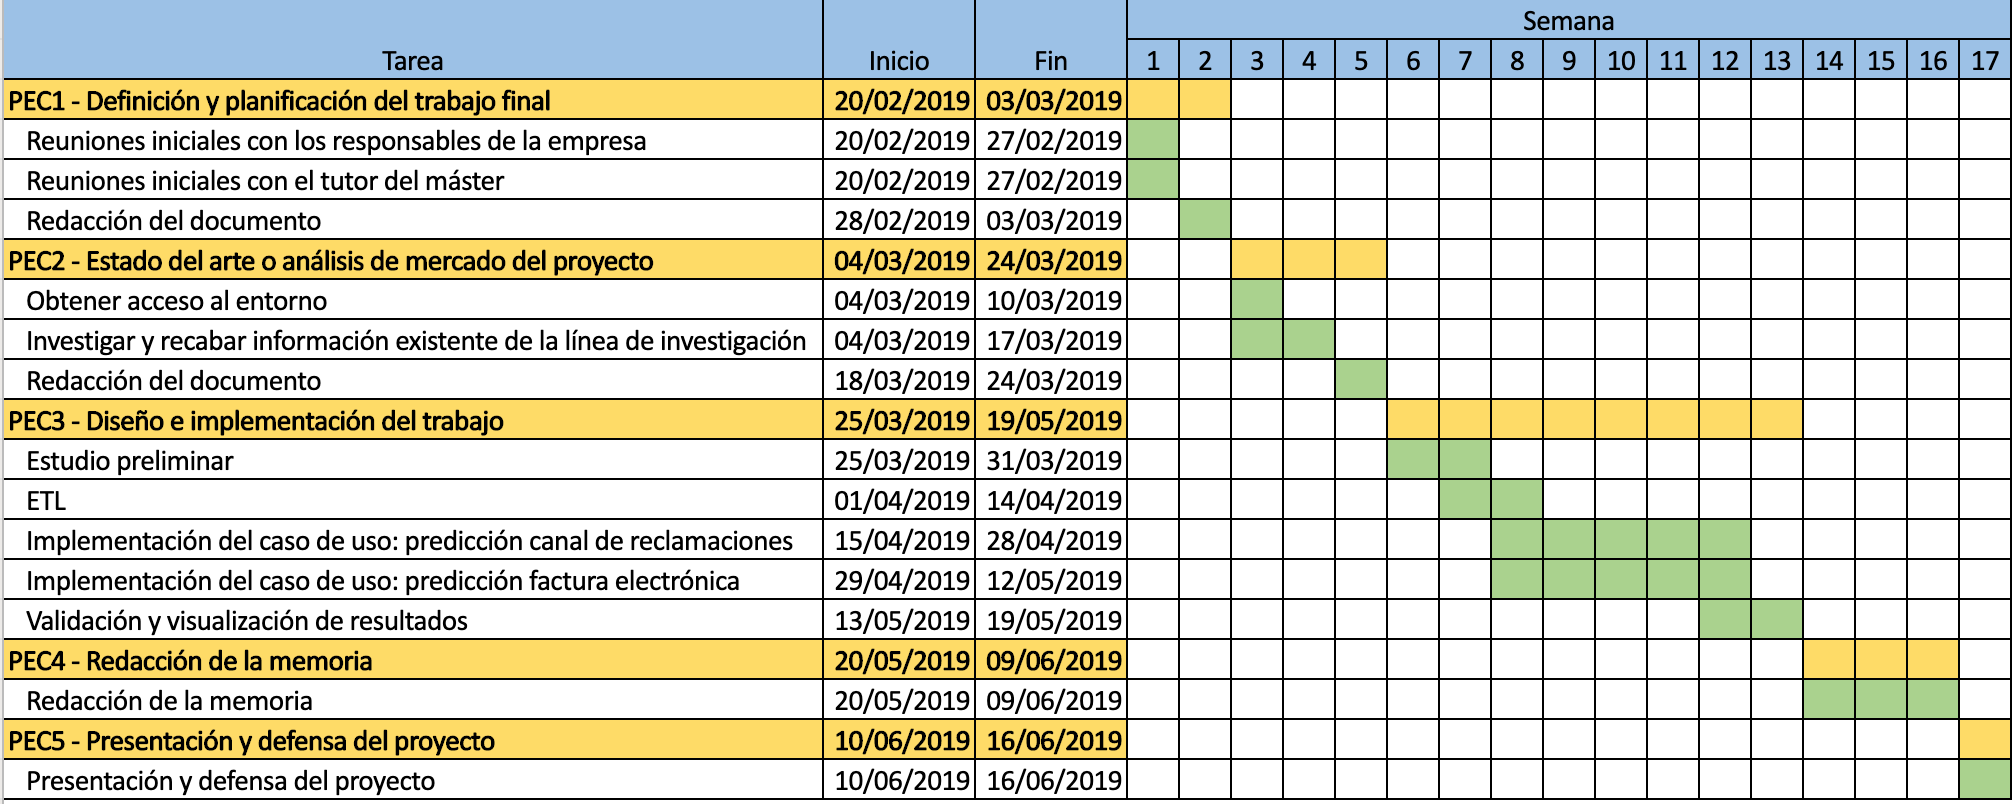
\includegraphics[width=1.0\textwidth]{TFM/figs/planificacion.png}}
\caption{Diagrama de Gantt que muestra la planificación del TFM}
\label{fig:planificacion}
\end{figure}

\subsection{Control de riesgos} 

Se han identificado dos riesgos potenciales que, por factores internos o externos, pueden alterar el curso de la planificación realizada para este TFM.  

Estos son los siguientes: 
\begin{itemize}
    \item Retraso en la obtención de accesos a la plataforma de \textit{``Big Data"}:
    
En el caso que no se disponga de la plataforma para la fase de “Diseño e implementación del trabajo”, se tomará la medida que eliminará tarea de implantación del caso de uso “Modelos de segmentación”. 
    \item Imposibilidad de poder aprovisionar información de clientes por motivos de GDPR:

Dado este caso, se tratará de hacer la segmentación de los clientes únicamente a partir de sus datos geopolíticos y de sus consumos.
\end{itemize}

\chapter{Estado del arte}
\label{chapter:estadodelarte}

En esta sección vamos a describir el panorama actual de \textit{``Big Data"}, las tecnologías que tenemos disponibles y los motivos de nuestra elección para la realización de este TFM.

%%% SECTION
\section{Big Data}
En los principios del siglo XXI las empresas tecnológicas como Google , Amazon y Yahoo tuvieron problemas para seguir prestando sus servicios como hasta ese momento, pues estaban almacenando una cantidad de información que luego sus servidores ya no podían procesar, por lo que debían usar un procesamiento paralelo para gestionar todos esos datos y así reducir el tiempo de procesamiento. Además, este problema se agravó porque aparecieron nuevas fuentes de información por lo que esta heterogeneidad de datos necesitó la creación de nuevos modelos de datos que facilitaran su proceso, sin importar su tipo o estructura. Por último, los datos necesitaban ser procesados de forma casi instantánea, por ejemplo en sus buscadores, para ofrecer un servicio óptimo para los clientes. 

Es por todo esto que se dieron cuenta que las técnicas tradicionales de procesamiento de datos no eran suficientes y se crearon nuevas tecnologías para poder continuar con el modelo de negocio que habían creado. 

Las nuevas técnicas para solventar los problemas descritos anteriormente se basaron en estos dos conceptos:
\begin{itemize}
    \item Dividir el problema en subproblemas de menor tamaño y complejidad. 
    \item Construir la solución final a partir del ensamblado de las soluciones parciales. 
\end{itemize}

Existen muchas definiciones de \textit{``Big Data"}, la primera definición del 2001 el analista Doug Laney de META Group (ahora Garner) utilizaba el término \textit{``Big Data"}\cite{laney} como el conjunto de técnicas y tecnologías para el tratamiento de datos, en entornos de gran volumen, variedad de orígenes y en los que la velocidad de respuesta es crítica - esta definición se conoce como las 3 V’s del \textit{``Big Data"}: volumen, velocidad y variedad.  

Posteriormente han surgido nuevas definiciones e incluso se han añadido más V’s a la definición original, como veracidad, valor, variabilidad, validez, volatilidad... 

Haciendo un resumen de todas estas interpretaciones sobre el mismo concepto, podemos quedarnos con la siguiente definición\cite{casas}: 

\textit{``Big Data"} es el conjunto de estrategias, tecnologías y sistemas para el almacenamiento, procesamiento, análisis y visualización de conjuntos de datos complejos.

%%% SECTION
\section{Cloud Computing}

El \textit{``Cloud Computing"}\cite{erl}\cite{skemp} o computación en la nube permite acceder a recursos informáticos desde cualquier lugar y en cualquier dispositivo compatible a través de Internet. La práctica se hizo popular durante los inicios del 2000 debido al amplio acceso a Internet y al aumento de la popularidad de dispositivos móviles como los teléfonos inteligentes. 

La computación en la nube evita la necesidad de instalar aplicaciones en dispositivos locales. En su nivel más básico, la computación en nube utiliza Internet para compartir recursos informáticos, como memoria, almacenamiento y potencia de procesamiento, y proporciona acceso a aplicaciones, datos y servicios desde cualquier lugar y en cualquier dispositivo. Algunos ejemplos puede ser Google Maps, Microsoft Word Online, Overleaf.

Las características que definen el \textit{``Cloud Computing"} son: Accesibilidad a Internet, configuración de recursos, multitenencia (una instancia de software que sirve a muchos usuarios), autenticación amplia, opciones de suscripción, funciones de autoservicio y accesibilidad desde cualquier lugar. 

Según la capa o el nivel de servicio que provee el \textit{``Cloud Computing"} nos encontraremos con los siguientes tipos: Infraestructure as a service, Platform as a service y Software as a service.

\subsection{Infraestructure as a service (IaaS)}

IaaS ofrece infraestructura de Cloud Computing a las organizaciones, incluyendo servidores, redes, sistemas operativos y almacenamiento, a través de la tecnología de virtualización. Estos servidores en nube se proporcionan normalmente al cliente a través de un panel o una API, y los clientes de IaaS tienen un control total sobre toda la infraestructura. IaaS proporciona las mismas tecnologías y capacidades que un centro de datos tradicional sin tener que mantenerlo o gestionarlo físicamente. Los clientes de IaaS todavía pueden acceder a sus servidores y almacenamiento directamente, pero todo se subcontrata a través de un "centro de datos virtual" en la nube. 

\subsection{Platform as a service (PaaS)}

Los servicios de plataforma en la nube proporcionan componentes de nube a cierto software mientras que se utilizan principalmente para aplicaciones. PaaS proporciona un marco de trabajo para los desarrolladores sobre el que pueden construir y utilizar para crear aplicaciones personalizadas. Todos los servidores, almacenamiento y redes pueden ser administrados por la empresa o por un proveedor externo, mientras que los desarrolladores pueden mantener la administración de las aplicaciones. 

\subsection{Software as a service (SaaS)}

Los servicios de aplicaciones en la nube utilizan Internet para entregar aplicaciones a sus usuarios, que son gestionadas por un proveedor externo. La mayoría de las aplicaciones SaaS se ejecutan directamente a través del navegador web y no requieren descargas o instalaciones en el lado del cliente.


%%% SECTION
\section{Hadoop}

Hadoop\cite{hadoop} es el framework de software libre que se encuentra en el corazón de gran parte de la revolución del Big Data y la analítica. Proporciona soluciones para el almacenamiento y análisis de datos empresariales con una escalabilidad lineal. 

La librería de software Apache Hadoop es un framework que permite el procesamiento distribuido de grandes conjuntos de datos a través de clusters de ordenadores utilizando modelos de programación simples. Está diseñado para pasar de servidores individuales a miles de máquinas, cada una de las cuales ofrece computación y almacenamiento local. En lugar de depender del hardware para ofrecer alta disponibilidad, la propia biblioteca está diseñada para detectar y gestionar los fallos en la capa de aplicación, ofreciendo así un servicio de alta disponibilidad sobre un grupo de ordenadores, cada uno de los cuales puede ser propenso a los fallos.

\subsection{Componentes}

Hadoop utiliza un sistema de ficheros distribuido (HDFS) que proporciona acceso de alto rendimiento a los datos de la aplicación y se basa en el paradigma MapReduce para el procesamiento en paralelo de grandes conjuntos de datos. Además, en su núcleo se encuentra YARN\cite{yarn}, un framework para la programación de trabajos y la gestión de recursos de clúster. 

Otros módulos muy importantes dentro del ecosistema de Hadoop son los siguientes: 
\begin{itemize}
    \item \textbf{Ambari}\cite{ambari}: Una herramienta basada en web para aprovisionar, gestionar y monitorizar clusters de Hadoop. 
    \item \textbf{Avro}\cite{avro}: Un sistema de serialización de datos. 
    \item \textbf{Cassandra}\cite{cassandra}: Una base de datos multi-master escalable sin puntos de fallo. 
    \item \textbf{HBase}\cite{hbase}: Una base de datos escalable y distribuida que soporta el almacenamiento estructurado de datos para grandes tablas. 
    \item \textbf{Hive}\cite{hive}: Una infraestructura de almacenamiento de datos que proporciona integración de datos y consultas ad hoc. 
    \item \textbf{Pig}\cite{pig}: Un lenguaje de flujo de datos de alto nivel y un marco de ejecución para el cálculo paralelo. 
    \item \textbf{Spark}\cite{spark}: Un motor de cálculo rápido y general para los datos de Hadoop. Spark proporciona un modelo de programación simple y expresivo que soporta una amplia gama de aplicaciones, incluyendo ETL, aprendizaje de máquinas, procesamiento de flujos y computación de gráficos. 
    \item \textbf{Tez}\cite{tez}: Un framework de programación de flujo de datos generalizado, construido sobre Hadoop YARN, que proporciona un motor potente y flexible para ejecutar un DAG arbitrario de tareas para procesar datos tanto para casos de uso por lotes como interactivos. 
    \item \textbf{ZooKeeper}\cite{zookeeper}: Un servicio de coordinación de alto rendimiento para aplicaciones distribuidas. 
    \item \textbf{Kafka}\cite{Kafka}: Un sistema para construir flujos de datos en tiempo real y aplicaciones en streaming. Es escalable horizontalmente, tolerante a fallos y rápido. 
    \item \textbf{Storm}\cite{storm}: Un sistema de computación en tiempo real. Facilita el procesamiento fiable de flujos de datos, haciendo para el procesamiento en tiempo real lo que Hadoop hizo para el procesamiento por lotes. 
\end{itemize}

\subsection{Distribuciones}

Hadoop, a pesar de ser un proyecto de software libre, cuenta con múltiples distribuciones comerciales que suministran este framework de Big Data como un paquete.  

Los más influyentes son las siguientes: 
\begin{itemize}
    \item \textbf{Cloudera}\cite{cloudera}

Cloudera fue el primer proveedor en ofrecer Hadoop como un paquete y continúa siendo líder en la industria. Su distribución Cloudera CDH, que contiene todos los componentes de código libre, es la distribución Hadoop más popular. Cloudera es conocida por innovar con adiciones a la estructura central, fue la primera en ofrecer SQL-for-Hadoop con su motor de consultas Impala. Otras aportaciones que incluyen son la interfaz de usuario, la seguridad y las interfaces para la integración con aplicaciones de terceros. Ofrece soporte para toda la distribución a través de su servicio de suscripción Cloudera Enterprise. 

    \item \textbf{Hortonworks}\cite{hortonworks}

La plataforma de Hortonworks es completamente de código libre,  de hecho, la compañía es conocida por hacer comprar otras compañías y liberar su código más útil en la comunidad de software libre. Lo que algunos han visto como el comienzo de una tendencia hacia la consolidación en el mercado ha provocado un crecimiento en la popularidad del producto de Hortonworks. Recientemente, Pivotal detuvo el desarrollo de su propia distribución y tanto Amazon como IBM están ofreciendo Hortonworks como opciones en sus propias plataformas, junto con sus propias distribuciones de Hadoop. La plataforma de Hortonworks también es el núcleo de la Open Data Platform Initiative, un grupo que busca simplificar y estandarizar las especificaciones en la ecosfera de Big Data. A largo plazo, es probable que esto signifique que recibirá un apoyo aún mayor.   

    \item \textbf{MapR}\cite{mapr}                              

Al igual que Hortonworks y Cloudera, MapR es un proveedor centrado en la plataforma, en lugar de un proveedor de servicios gestionados. MapR integra su propio sistema de base de datos MapR-DB que, según afirman, es entre cuatro y siete veces más rápido que la base de datos Hadoop HBase que se ejecuta en distribuciones de la competencia. Debido a su potencia y velocidad, MapR se considera a menudo una buena opción para los proyectos más grandes y exigentes de Big Data. 

    \item \textbf{Amazon Elastic Map Reduce}\cite{amazonemr}

Amazon ofrece una plataforma Hadoop-as-a-Service bajo el brazo de Amazon Web Services. Una ventaja clave del modelo de pago \textit{“pay-as-you-go"} que ofrecen los proveedores de servicios exclusivamente en la nube es la escalabilidad que ofrecen, ya que el almacenamiento y el procesamiento de datos pueden ampliarse o reducirse a medida que cambia la demanda. Amazon ha anunciado recientemente que los clientes pueden ahora utilizar el framework de procesamiento de flujos Apache Flink para el análisis de datos en tiempo real, junto con otras herramientas populares como Kafka y Presto. También se conecta sin problemas con otras infraestructuras de servicios en la nube de Amazon, como EC2 para el procesamiento en la nube, Amazon S3 y DynamoDB para el almacenamiento y AWS IoT para recopilar datos de los dispositivos del IoT (Internet de las cosas). 

    \item \textbf{Microsoft}\cite{microsofthdinsight}

La plataforma Azure HDInsight de Microsoft es un servicio en la nube que ofrece instalaciones gestionadas de varias distribuciones Hadoop de código abierto, incluyendo Hortonworks, Cloudera y MapR. Los integra con su propia plataforma Azure Data Lake para ofrecer una solución completa de almacenamiento y análisis basados en la nube. Además del framework central de Hadoop, HDInsights proporciona servicios de nube de Spark, Hive, Kafka y Storm, y su propio marco de seguridad de la nube. 

    \item \textbf{Altiscale}\cite{altiscale} 

Adquirida recientemente por SAP por un valor de 125 millones de dólares, Altiscale es otra empresa que ofrece un servicio de Hadoop-as-a-service gestionado y basado en la nube. Su producto Altiscale Data Cloud incluye servicios operativos adicionales como automatización, seguridad, escalado y ajuste de rendimiento junto con el marco central de Hadoop. Altiscale Data Cloud también proporciona servicios gestionados de Spark, Hive y Pig pero a diferencia de los otros, utiliza su propia distribución de Hadoop en lugar de la de uno de los proveedores centrados en la plataforma, como Hortonworks o MapR.
\end{itemize}

Cabe destacar que recientemente (30 de octubre de 2018) se anunció la unión de las dos principales distribuciones, Cloudera y Hortonworks, aunque a día de hoy todavía se mantienen como distribuciones distintas.

%%SECTION
\section{Comparativa de las diferentes arquitecturas}

Hadoop se puede clasificar en tres variantes según la tipología de su arquitectura\cite{bengfort}.

\subsection{Plataformas Cloud}

El modelo basado en la nube permite la mejor adaptabilidad a la vez que proporciona un cifrado de alta seguridad de los datos tanto en reposo como en tránsito. Este modelo permite actualizaciones fuera de horario que no causarán interrupciones en la funcionalidad. Además, la nube está lista para desplegarse en mucho menos tiempo que los otros modelos, mientras que su coste es por licencia de usuarios\cite{havanki}.

\subsection{Plataformas Híbridas}

El modelo híbrido es ideal para aquellas empresas que requieren un grado ligeramente superior de seguridad sobre el modelo basado en la nube. El híbrido crea un puente cifrado entre el hardware interno que alberga datos internos y la nube externa que ayuda a organizar la información externa y analizarla. Una vez que el hardware adicional está en su lugar, no se necesita más tiempo para su implementación que un simple modelo de nube y proporciona mayor seguridad a la vez que mantiene la adaptabilidad, pero con un mayor coste. 

\subsection{Plataformas On Premise}

El modelo \textit{``On Premise"} es con diferencia el más costoso y lento de implementar, ya que todas las herramientas necesarias deben estar en las instalaciones. El equipo requerido hace que esta opción sea generalmente prohibitiva en términos de coste, pero proporciona un alto nivel de seguridad. En principio, carece de la adaptabilidad de los modelos anteriores y tarda mucho más tiempo en actualizarse. Este debería ser un modelo de último recurso para aquellos que están fuertemente regulados lejos de cualquier tipo de modelo híbrido o de nube.

%%% SECTION
\section{Entorno de trabajo}

En mi compañía se ha optado por contratar los servicios \textit{``Cloud"} de Microsoft, por lo que contaremos con la distribución de Hadoop en la plataforma Azure HDInsight\cite{yadav}. En concreto, esta plataforma está basada en la distribución de Hadoop de Hortonworks.

El motivo de la selección de esta distribución ha sido porque, además de contar con los servicios de una empresa como Microsoft, disponer de una infraestructura \textit{``Cloud"} tipo IaaS para el entorno Hadoop permite una mayor flexibilidad y escalabilidad que los otros sistemas \textit{``On Premise"}. Es muy rápido el proceso de crear, eliminar nodos, modificar sus características, así como aumentar el espacio de almacenamiento. 

\subsection{Caracerísticas}
Las características que compenen el entorno de trabajo son las siguientes:
\begin{itemize}
    \item Versión:

La versión de HDInsight es la 3.6 que se corresponde con la versión 2.6 de Hortonworks Data Platform (HDP). 

    \item Nodos:

2 Head (28 GB RAM) 
4 Workers (56 GB RAM) 
3 Zookeepers (4 GB RAM) 

    \item Almacenamiento:

En el almacenamiento HDFS disponemos de 1,5 TB, mientras que en el Data Lake se dispondrá de un espacio altamente escalable, pues se factura mensualmente por el espacio usado mediante el sistema pay-as-you-go. 
\end{itemize}

\subsection{Datos}

Los datos iniciales están alojados en el Data Lake de Azure y son aprovisionados diariamente de la información que reside en el repositorio informacional Oracle EXADATA. 

Contaremos con las siguientes tablas: 

\begin{itemize}
    \item DATOS\_WEB: 300.642.104 registros - 362 GB 

    Registro de todas las interacciones realizadas por los clientes en las plataformas web del Portal del Cliente y en las aplicaciones móviles. 

    \item FACTURA: 590.473.454 registros - 74 GB 

    Datos de facturación mensual/bimensual de cada cliente. 

    \item CONSUMO: 837.014.368 registros - 16 GB 

    Detalle del consumo de los clientes. 

    \item RECLAMACION: 3.218.571 registros - 1.2 GB 

    Reclamaciones realizadas por los clientes. 

    \item ACCION\_CLIENTE: 133.026.680 registros - 7,5 GB 

    Acciones realizadas al cliente: altas, bajas, cambio de titularidad... 

    \item INTERACCION\_CLIENTE: 113.969.367 registros - 3,4 GB 

    Interacciones realizadas con el cliente: por teléfono, email, puntos de atención... 

    \item CALLBACK\_CLIENTE: 4.767.664 registros - 500 MB 

    Registro de llamadas tipo Callback al cliente. 

    \item CLIENTE: 15.242.851 registros - 2,2 GB 

    Información personal del cliente. 

    \item CONTRATO: 30.421.621 registros - 7,1 GB 

    Información relativa al contrato entre la empresa y el cliente. 

    \item DIRECCION\_CLIENTE: 29.212.542 registros – 1,9 GB 

    Información del domicilio del cliente. 
\end{itemize}

\chapter{Aspectos de diseño y desarrollo}
\label{chapter:disenyo_y_desarrollo}


%%% SECTION
\section{Aspectos de diseño}
El planteamiento inicial de este proyecto, en lo que se refiere al diseño, fue realizarlo íntegramente en el entorno de \textit{``Big Data"} Azure HDInsight.
Puesto que este entorno todavía tiene carencias por estar en una fase temprana de despliegue, nos hemos apoyado también en el entorno ``Databricks Community Edition"\cite{databricks}, visto en el laboratorio de la asignatura de ``Análisis de datos en entornos Big Data".

A continuación describiremos las distintas fases que se van a realizar a lo largo del desarrollo del proyecto.

\subsection{Estudio preliminar}
Esta fase va a ser el punto de partida para el resto del trabajo, vamos a tratar de entender el negocio así como la intención de los retos propuestos.
Además, focalizaremos nuestra atención en la comprensión de los datos y la determinación de los requerimientos de información necesarios para poder llevar a cabo nuestro proyecto.

\subsection{Tratamiento y saneamiento de los datos}
Una vez los recursos de datos están identificados, es necesario que sean seleccionados, limpiados, transformados a la forma deseada y formateados. En esta fase se llevará a cabo los procesos de transformación y limpieza de datos, necesarios para el posterior modelado.
Como partimos de unos datos que ya están cargados en el almacenamiento del cluster de Big Data, no tendremos que preocuparnos por la carga de estos desde otros sistemas.
El objetivo de esta fase será, conseguir varias tablas enriquecidas con la información otras tablas para que luego nos sirva para entrenar nuestro modelo y obtener predicciones.
Es por esto que tendremos que seleccionar los atributos que veamos que pueden ser interesantes a la vez que crear datos agregados que puedan suponer un valor añadido.
Por otra parte, deberemos sanear esos datos para luego facilitar las fases de creación y entrenamiento de los modelos predictivos. Estas tareas de adecuación las podemos agrupar en: tareas de limpieza, normalización, discretización y reducción de la dimensionalidad.  

\begin{enumerate}
    \item Limpieza de datos:
    
En este proceso se llevan a cabo actividades de detección, eliminación o corrección de valores inapropiados en el conjunto de datos. Se pretende detectar y subsanar los errores de forma que obtengamos unos datos lo más completos y consistentes posible.

    \item Normalización de datos:
    
En la normalización de datos trataremos de lograr que los datos estén en una escala de valores equivalentes para simplificar la comparación entre ellos.

La normalización es útil para varios métodos de minería de datos, de forma que reducimos la influencia de los atributos con valores más altos y que pueden distorsionr el resultado del modelo.


Existen varios métodos de normalización, como la normalización por el máximo, por la diferencia y por la desviación estándar.

    \item Discretización de datos:
    
    
En la discretización cambiaremos los valores de una variable continua en contenedores, intervalos o grupos, para limitar el número de estados posibles. 
De esta forma podremos tratar a los contenedores como si fueran categorías.
Los métodos de discretización se pueden clasificar en estas tres categorías:
\begin{itemize}
    \item Supervisados o no supervisados.
    \item Locales o globales.
    \item Parametrizados y no parametrizados.
\end{itemize}

    \item Reducción de la dimensionalidad:
    
En la reducción de la dimensionalidad reduciremos el número aleatorio de variables para obtener un conjunto de variables principales manteniendo el nivel de calidad necesario. Está dividido en dos tipos, selección de atributos y extracción de atributos.

\end{enumerate}

\subsection{Exploración y análisis de los datos}
La exploración y análisis de los datos o EDA (acrónimo  de \textit{``Exploratory Data Analysis"}) es importante y recomendada en los pasos previos al entrenamiento del modelo de \textit{``machine learning"}. Estas tareas se basan en el uso de cuadros resumen y herramientas gráficas que permiten detectar visualmente la distribución de los datos, la presencia de valores extremos y las relaciones entre los atributos.

\subsection{Creación y entrenamiento del modelo predictivo}
En esta sección, crearemos diferentes tipos de modelos para luego poder compararlos y elegir el que mejores resultados nos ofrezca o el que mejor se adapte a las condiciones de nuestro entorno.
Previamente a la creación del modelo dividiremos el conjunto de datos en dos bloques, uno para entrenar el modelo y otro para validar la precisión de los resultados.
De esta forma evitaremos que nuestro modelo se sobreentrene (en inglés, \textit{overfitting} y sea independiente de los datos utilizados en el entrenamiento.
Esto tiene sentido hacerlo porque nuestro modelo es de aprendizaje supervisado, para otros modelos que no son de este tipo no es necesario realizar esta división de los datos.

\subsection{Validación y visualización de los resultados}
Una vez tenemos nuestro modelo creado y entrenado pasaremos al último paso que es la validación. 
Con el otro conjunto de datos que no hemos utilizado para el entrenamiento, lo usaremos para realizar las predicciones de forma que podamos comparar la predicción del modelo con el resultado real.

Para esta evaluación de los resultados nos apoyaremos de métricas e indicadores que puedan cuantificar la precisión del modelo, permitiendo la comparación entre distintos métodos sobre el mismo conjunto de datos.

Existen distintas métricas específicas para los problemas de clasificación, regresión o agrupamiento.
En nuestro caso vamos a tratar de problemas de clasificación, por lo que las métricas que usaremos será la matriz de confusión y otras métricas derivadas de esta.

\subsubsection{Matriz de confusión}
La matriz de confusión (confusion matrix) muestra gráficamente los aciertos y errores cometidos por el modelo de clasificación. 
\begin{figure}[H]
\centerline{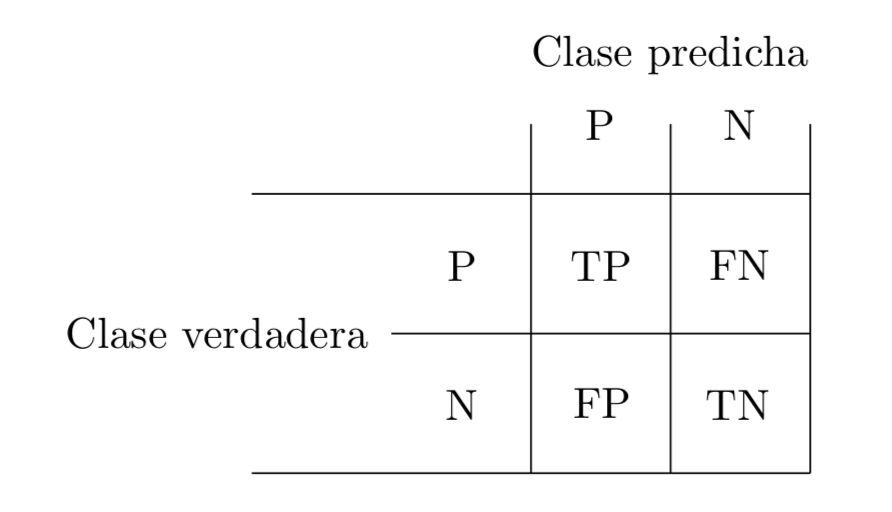
\includegraphics[width=0.5\textwidth]{TFM/figs/matrizconfusion.png}}
\caption{Matriz de confusión binaria}
\label{fig:matrizconfusion}
\end{figure}
Los parámetros que nos indica son:
Verdadero positivo (\textit{True Positive}, TP): número de clasificaciones correctas en la clase positiva (P).
Verdadero negativo (\textit{True Negative}, TN): número de clasificaciones correctas en la clase negativa (N).
Falso negativo (\textit{False Negative}, FN): número de clasificaciones incorrectas de clase positiva clasificada como negativa.
Falso positivo (\textit{False Positive}, FP): número de clasificaciones incorrectas de clase negativa clasificada como positiva.

\subsubsection{Métricas derivadas de la matriz de confusión}
A partir de la matriz de confusión, podemos obtener un conjunto de métricas que permiten cuantificar la bondad de un modelo de clasificación.
Podemos definir las siguientes:
\begin{itemize}
    \item Exactitud (\textit{accuracy}, ACC): número de predicciones correctas sobre el número total de predicciones.
    \begin{equation}
    ACC=\frac{TP+TN}{FP+FN+TP+TN}
    \end{equation}
    \item Error de clasificación (\textit{misclassification error}, ERR): número de predicciones incorrectas sobre el número total de predicciones.
    \begin{equation}
    ERR=\frac{FP+FN}{FP+FN+TP+TN}=1-ACC
    \end{equation}
    \item Tasa de verdaderos positivos (\textit{True Positive Rate}, TPR): tasa de acierto en los verdaderos positivos.
    \begin{equation}
    TPR=\frac{TP}{FN+TP}
    \end{equation} 
    \item Tasa de verdaderos negativos (\textit{False Positive Rate}, FPR): tasa de error en los falsos positivos.
    \begin{equation}
    FPR=\frac{FP}{FP+TN}
    \end{equation}
    \item Precisión (\textit{precision}, PRE): relaciona las tasas de verdaderos positivos y negativos.
    \begin{equation}
    PRE=\frac{TP}{FP+TP}
    \end{equation}
    \item Sensibilidad (\textit{recall}, REC): tasa de acierto en los verdaderos positivos.
       \begin{equation}
    REC=\frac{TP}{FN+TP}=TPR
    \end{equation}
    \item Especificidad (\textit{specificity}, SPE): tasa de instancias correctamente clasificadas como negativas respecto a todas las instancias negativas.
    \begin{equation}
    SPE=\frac{TN}{FP+TN}=1-FPR
    \end{equation}
    \item F1 (\textit{F1 score}): combina la precisión y la sensibilidad.
    \begin{equation}
    F1=2\times\frac{PRE \times REC}{PRE+REC}
    \end{equation} 
    
\end{itemize}

\subsubsection{Curva ROC}
Una curva ROC (acrónimo de \textit{Receiver Operating Characteristic}) mide el rendimiento respecto a los falsos positivos (FP) y verdaderos positivos (TP).
\begin{figure}[H]
\centerline{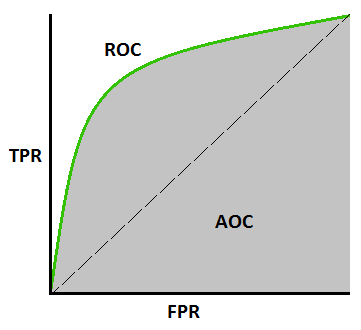
\includegraphics[width=0.5\textwidth]{TFM/figs/roc.png}}
\caption{Curva ROC}
\label{fig:roc}
\end{figure}

En esta métrica, se puede ver que cuanto más pegada esté la curva a la esquina superior izquierda del gráfico mejor clasificador será.

A partir de esta curva, podemos calcular el área bajo la curva (\textit{area under the curve}, AUC) que muestra el rendimiento del modelo de clasificación.



%%% SECTION
\section{Desarrollo}

En este apartado vamos a describir los pasos que hemos realizado para elaborar los objetivos que se plantearon al inicio del proyecto.

Todo el código fuente elaborado para el desarrollo de estos objetivos para se puede encontrar en el repositorio  \href{github}{https://github.com/dieconji/tfm/tree/master/code}.


\subsection{Análisis previo}
El objetivo principal era conocer qué funcionalidades en las plataformas digitales permiten la reducción de llamadas telefónicas recibidas.

Tras analizar los datos disponibles, se ha tomado la decisión de dividir este objetivo principal en dos modelos, de forma que con la ayuda de estos dos seamos capaces de obtener el conocimiento que se sugiere en la misión principal.
El motivo de necesitar dividir este objetivo es porque con los datos que tenemos no se puede cuantificar la precisión de nuestro modelo, ya que los resultados finales no se pueden contrastar con la realidad si no la conocemos.

Así pues, los dos objetivos que vamos a plantear son los siguientes:
\begin{itemize}
    \item Predicción del canal por el que se ha realizado una reclamación:
    
    La misión de este modelo va a ser predecir si la reclamación que ha realizado un cliente ha sido por las plataformas digitales o por otros canales
    \item Predicción de facturación electrónica:
    
    Con este modelo podremos predecir, dado un cliente si tiene facturación electrónica o no.
\end{itemize}


\subsection{Creación de tablas minables}
Como nuestro objetivo es obtener dos modelos analíticos predictivos distintos, tenemos que plantearnos qué tipo de información vamos a necesitar para cada uno de ellos.

Así pues, tras estudiar el conjunto de datos y analizar los retos propuestos se ha decidido la creación de dos tablas minables distintas, creadas a partir de la información disponible, de modo que cada una de ella sirva para crear, entrenar y validar cada objetivo.
Estas tablas serán las siguientes:
\begin{itemize}
    \item Cliente: Cada registro pertenece a un cliente/contrato. Esta tabla está  enriquecida con información sobre su facturación, sobre las acciones que ha realizado en distintos canales y sobre sus sesiones en las plataformas digitales.
    \item Acción: Cada registro pertenece a una acción de tipo reclamación. Está enriquecida con la información del cliente, facturación del cliente y sesiones en las plataformas digitales.
\end{itemize}

Estas tablas van a compartir información en común, el inicio de creación de ambas tablas va a ser compartido pero el formato y características obliga a que se tengan que tomar varios caminos para la creación final de cada una.

Inicialmente se intentó generar esta información directamente desde el entorno Big Data con el uso de Zeppelin\cite{zeppelin}, pero ocasionó muchos problemas varios motivos:
\begin{itemize}
    \item Apagado automático del cluster los fines de semana:
    
    Por motivos económicos, los clusters de HDInsights estaban programados para eliminarse los fines de semana y volver a crearse el lunes a primera hora. Esto es una de las ventajas de los entornos cloud de Big Data, pero que nos ha ocasionado más problemas de los previstos inicialmente. 
    \item Fallos operativos en el entorno de \textit{notebooks} Zeppelin:
    
    Tras haber trabajado con los \textit{notebooks} de Jupyter\cite{jupyter} y Databricks, la idea de trabajar con Zeppelin parecía la más adecuada. Sin embargo, en esta instalación que disponíamos fallaba cada vez que se cancelaba una consulta, de forma que el servicio se quedaba bloqueado hasta que se reiniciara el servicio. El usuario que tenía disponible carecía de tales permisos, por lo que había que lanzar una incidencia y esperar que la tramitasen hasta varios días después.
\end{itemize}

Tras estos problemas iniciales se optó por trabajar con \textit{scripts Pyhton}\cite{python}. Además, como el tiempo de ejecución de la mayoría de las consultas era muy elevado, además de limitar el tamaño de las tablas para las pruebas iniciales, se utilizó la aplicación \textit{nohup}\cite{nohup} para poder dejar ``en ejecución" una consulta en \textit{background} y no depender de tener la sesión abierta.

De esta forma para cada operación de cruce entre tablas o enriquecimiento en el \textit{script} se modeló de la forma siguiente:
\begin{itemize}
    \item Insertar un registro en la tabla log de la BBDD con la fecha y título de la operación.
    \item Borrar tabla persistente en caso de existir.
    \item Crear un \textit{dataframe} a partir de la consulta SQL en la tabla.
    \item Crear una tabla temporal en la BBDD con la información del \textit{dataframe}.
    \item Crear una tabla persistente a partir de la temporal
\end{itemize}

Un ejemplo de código de una operación sería el siguiente:

\begin{minipage}{\linewidth}
\begin{lstlisting}[language=Python, caption=Ejemplo de operación en la creación de las tablas minables]
### FACTURAS
sqlContext.sql("insert into u257030.log select current_timestamp() fecha , 'FACTURAS' operacion")
facturas_df = sqlContext.sql("SELECT cod_cliente, cod_contrato, avg(imp_total_factu) as importe_medio FROM dwvp.ghh_factura GROUP BY cod_cliente, cod_contrato")
sqlContext.sql("DROP TABLE IF EXISTS u257030.facturas_df")
facturas_df.createOrReplaceTempView("tmp_facturas_df")
sqlContext.sql("CREATE TABLE u257030.facturas_df USING PARQUET AS SELECT * FROM tmp_facturas_df")
\end{lstlisting}
\end{minipage}  


Una vez obtenidas las tablas finales, enriquecidas con todos los campos que pueden aportar valor, las exportamos en ficheros CSV para poder tratarlas en Databricks. Como las tablas finales eran muy pesadas se hicieron descargas con registros limitados para hacer poder manejarlos de una manera más cómoda.

Todo el ciclo de vida del proyecto se pretendió gestionarlo íntegramente en el entorno HDInsight, pero dados los problemas detectados se consideró continuar el desarrollo en Databricks. De esta forma podríamos trabajar con un entorno notebook que nos permitiera trabajar de una forma mucho más ágil y cómoda que el entorno que se eligió en un inicio.

\subsection{Limpieza de datos}
Tras la importación de las tablas minables en Databricks se continuó con la limpieza de los datos.
Aquí primero se realizaron las siguientes procesos:
\begin{itemize}
    \item Tratar los valores vacíos o nulos:
    En el caso de campos categóricos añadiendo una nueva categoría con el valor 'NULO' y para los numéricos la media y la creación de un campo nuevo binario para indicar si era o no nulo.
    \item Normalizar las fechas:
    Se cambia de String/Timestamp a tipo Integer con el formato YYYYMMDD.
    \item Normalizar los campos numéricos a valores entre 0 y 1.
    \item Codificar las variables categóricas a columnas binarias con el método OneHotEncoder.
\end{itemize}

\subsection{Creación de los modelos}
Una vez ya tenemos los datos saneados podemos comenzar con la generación de modelos.

Para esto dividiremos nuestro \textit{dataset} en dos conjuntos, un 70\% para el entrenamiento y un 30\% para las validaciones.

Los modelos predictivos que se realizaron son en ambos casos de la tipología categorización, y fueron de los siguientes métodos:
\begin{itemize}
    \item Logistic Regression\cite{lr}.
    
La regresión logística es un método popular para predecir una respuesta categórica. Es un caso especial de los modelos \texit{`Generalized Linear models'} que predicen la probabilidad de las salidas. Este método puede ser usado tanto para predecir una salida binaria como para predecir una salida multiclase.

    \item Decision Tree Classifier\cite{dtc}.
    
Los árboles de decisión son unos métodos populares de la familia de clasificación y regresión.
Están ampliamente extendidos por su facilidad de interpretar, manejar características categóricas, extender a la clasificación multiclase, y son capaces de capturar no linealidades y interacciones de características.

    \item Random Forest Classifier\cite{rfc}.
    
Los clasificadores \textit{``Random Forests"} son conjuntos de árboles de decisión, cominándolos de forma que se reduce el riesgo de sobreentreamiento.

    \item Gradient-boosted Tree Classifier\cite{gbt}.
    
Los clasificadores \textit{``Gradient-boosted Tree"} entrenan iterativamente árboles de decisión en orden de minimizar la función de pérdida o \textit{``loss"}.

    \item Linear Support Vector Machine\cite{lsvm}.
    
Una máquina de soporte vectorial construye un hiperplano o conjunto de hiperplanos en un espacio de dimensiones muy altas o infinitas que pueden ser usadas para tareas de clasificación, regresión, u otras tareas. Instintivamente, una buena separación se consigue por el hiperplano que tiene mayor distancia a los puntos más cercanos de los datos de entreamiento de cualquier clase, en general, a mayor margen menor error de generalización del clasificador.

\end{itemize}

Para cada uno de ellos, el procedimiento de creación, entrenamiento y generación de predicciones ha sido el mismo.
Este es un ejemplo de cómo se ha generado el modelo de Gradient-boosted Tree Classifier:

\begin{minipage}{\linewidth}
\begin{lstlisting}[language=Python, caption=Métricas derivadas de la matriz de confusión]
from pyspark.ml.classification import GBTClassifier

# creamos el modelo
gbt = GBTClassifier(maxIter=10)

# entrenamos el modelo
gbtModel = gbt.fit(train)

# obtenemos las predicciones del conjunto test
predictions = gbtModel.transform(test)
\end{lstlisting}
\end{minipage}  

Por último, para poder medir la calidad de cada modelo nos hemos ayudado de los siguientes elementos:

\begin{itemize}
\begin{minipage}{\linewidth}
    \item Matriz de confusión

\begin{lstlisting}[language=Python, caption=Matriz de confusión]
from sklearn.metrics import confusion_matrix

def matriz_confusion(y_true, y_pred):
  # nombre de las clases
  class_names = [0, 1]

  # creamos matriz de confusion
  cnf_matrix = confusion_matrix(y_true, y_pred, labels=class_names)
  
  # normalizamos
  cm = cnf_matrix.astype('float') / cnf_matrix.sum(axis=1)[:, np.newaxis]
  
  # mostramos matriz de confusion
  plt.imshow(cm, interpolation='nearest', cmap=plt.cm.Blues, aspect="auto")
  plt.title('Matriz de confusion normalizada')
  plt.colorbar()
  tick_marks = np.arange(len(class_names))
  plt.xticks(tick_marks, class_names, rotation=45)
  plt.yticks(tick_marks, class_names)

  thresh = cm.max() / 2.
  for i, j in itertools.product(range(cm.shape[0]), range(cm.shape[1])):
      plt.text(j, i, format(cm[i, j], '.2f'),
               horizontalalignment="center",
               color="white" if cm[i, j] > thresh else "black")

  plt.tight_layout()
  plt.ylabel('Clase verdadera')
  plt.xlabel('Clase predicha')
\end{lstlisting}
\end{minipage}  

\begin{minipage}{\linewidth}
    \item Métricas derivadas de la matriz de confusión

\begin{lstlisting}[language=Python, caption=Métricas derivadas de la matriz de confusión]
def mostrar_metricas(predictions):
  # devuelve las clases
  y_true = predictions.select("label")
  y_true = y_true.toPandas()

  # devuelve las predicciones
  y_pred = predictions.select("prediction")
  y_pred = y_pred.toPandas()

  # obtenemos la matriz de confusion
  TN, FP, FN, TP = confusion_matrix(y_true, y_pred).ravel()
  
  # cambiamos el tipo a float
  FP = FP.astype(float)
  FN = FN.astype(float)
  TP = TP.astype(float)
  TN = TN.astype(float)

  # obtenemos las metricas
  REC = TP/(TP+FN)
  SPE = TN/(TN+FP) 
  PRE = TP/(TP+FP)
  FPR = FP/(FP+TN)
  ACC = (TP+TN)/(TP+FP+FN+TN)
  ERR = 1-ACC
  F1 = 2*(PRE*REC)/(PRE+REC)
  evaluator = BinaryClassificationEvaluator()
  AUROC = evaluator.evaluate(predictions, {evaluator.metricName: "areaUnderROC"})
  
  # mostramos las metricas
  print('Exactitud (ACC): {:.2f}'.format(ACC))
  print('Error de clasificacion (ERR): {:.2f}'.format(ERR))
  print('Tasa de verdaderos positivos o sensibilidad (TPR | REC): {:.2f}'.format(REC))
  print('Tasa de verdaderos negativos (FPR): {:.2f}'.format(FPR))
  print('Precision (PRE): {:.2f}'.format(PRE))
  print('Especificidad(SPE): {:.2f}'.format(SPE))
  print('F1: {:.2f}'.format(F1))  
  print('Area bajo la curva ROC: {:.2f}'.format(AUROC))
\end{lstlisting}
\end{minipage}

\begin{minipage}{\linewidth}
    \item Curva ROC

\begin{lstlisting}[language=Python, caption=Curva ROC]
from sklearn.metrics import roc_curve  

def curva_roc(y_true, y_pred):
  # obtenemos ratio de falsos positivos y verdaderos positivos
  fpr, tpr, thresholds = roc_curve(y_true, y_pred)

  # mostramos la curva
  plt.plot(fpr, tpr, color='orange', label='ROC')
  plt.plot([0, 1], [0, 1], color='darkblue', linestyle='--')
  plt.xlabel('Ratio de Falsos Positivos')
  plt.ylabel('Ratio de Verdaderos Positivos')
  plt.title('Curva ROC')
  plt.legend()
  plt.tight_layout()
\end{lstlisting}
\end{minipage}
\end{itemize}
\chapter{Experimentos y resultados}
\label{chapter:experimentos_y_resultados}
En este capítulo vamos a comentar los experimentos realizados para cada objetivo y los resultados obtenidos.

%%% SECTION
\section{Experimentos}
Los experimentos realizados en este TFM han sido modelados y ejecutados íntegramente en el entorno \textit{``Big Data"} de Databricks Community Edition, tanto para el objetivo de predecir la facturación de los clientes, como para la predicción del canal por el que se ha realizado una reclamación. Seguidamente describiremos por separado cada uno de ellos.

\subsection{Predicción de facturación electrónica de los clientes}

El conjunto de datos cargado en la plataforma contaba con 1.000.000 registros de clientes. El conjunto era mayor en un inicio, pero por restricciones de espacio en la versión gratuita de Databricks se hizo un filtrado previo.
Todos los clientes tienen informado el campo que determina si la facturación se le envía por vía correo postal o por correo electrónico, así que podemos usar todo el \textit{dataset} sin necesidad de filtros adicionales.


Tras realizar un análisis exploratorio de los datos, vemos que la cantidad de clientes que tienen un u otro estado no es proporcionado, pues es más de cinco veces mayor la cantidad de clientes que tienen facturación por correo postal de los que tienen facturación electrónica.
Esto se conoce como datos desbalanceados (\textit{``imbalanced data"} en inglés), y ocurre en los problemas de clasificación cuando en nuestros datos de entrenamiento tenemos alguna clase minoriataria. Este problema puede conllevar una bajada calidad en nuestros modelos, ya que se entrenarían con datos mayoritariamente de una clase y aprenderían más de una que de otra. Incluso pueden llegar a simplificar la clasificación determinando que la predicción siempre es de la clase mayoritaria obteniendo buenos resultados en la precisión.
Por ejemplo, en este mismo caso que estamos tratando donde una clase es cinco veces mayor que la otra la precisión de este tipo de modelo sería del 80\%.

Para tratar el problema de datos desbalanceados existen varios métodos:
\begin{itemize}
    \item Undersampling:
    
    \textit{``Undersampling"} es el proceso donde aleatoriamente se eliminan algunas de las observaciones de la clase mayoritaria hasta hacerla coincidir con el número de observaciones de la clase minoritaria.
    
    \item Oversampling:
    
    \textit{``Oversampling"} es un proceso más complejo que el anterior y se basas en generar datos sintéticos a partir de las observaciones de la clase minoritaria.
    Hay una gran variedad de métodos usados para este proceso, pero el más común es el llamado SMOTE (acrónimo en inglés de \textit{``Synthetic Minority Over-sampling Technique"}).

    \item Ensemble Classifiers:
    
    Utiliza las ventajas de hacer un ensamblado de métodos de clasificación, es decir, entrena diversos modelos y entre todos obtiene el resultado final (como un sistema democrático de votaciones) pero se asegura de tomar muestras de entrenamiento equilibradas.
    
\end{itemize}

Para prevenir que esta desproporción pueda afectar a la calidad de los modelos y dado que disponemos de un conjunto de datos todavía considerable, se decide hacer un \textit{``Undersampling"} tomando una muestra aleatoria de 150.000 registros de cada tipo y juntándolos en un nuevo \textit{dataset} de 300.000 registros en total.


\subsection{Predicción del canal por el que se ha realizado una reclamación}

Para el caso de la predicción del canal de reclamaciones y quejas no fue necesario realizar un filtrado de los datos para cargarlos en el entorno de Databricks, ya que este conjunto de datos es una división del resto de acciones de los clientes con la empresa y en total sumaba 448.589 registros.

Como sucedió en el caso anterior, la cantidad de casos de una u otra tipología es desproporcionada. Casi cuatro veces mayor son las reclamaciones realizadas por plataformas no digitales de las que sí lo son.
Igual que con el \textit{dataset} de clientes, para prevenir una pérdida en la calidad de los modelos, se tomará una muestra aleatoria de 90.000 registros de cada tipo y se juntarán en nuevo conjunto de datos de 180.000 registros en total.

%%% SECTION
\section{Resultados}

A continuación mostraremos los resultados de los modelos  para cada uno de estos objetivos, de los cinco tipos distintos de clasificación.

\subsection{Predicción de facturación electrónica de los clientes}

Como veremos a continuación en el detalle de cada modelo de predicción, los modelos han obtenido para este objetivo una buena calidad en sus predicciones, con una exactitud y un F1 en torno al 0.85 en la mayoría de ellos.

\begin{itemize}

%\begin{minipage}{\linewidth}
    \item Logistic Regression

El modelo de regresión logística ha obtenido un buena calidad como podemos ver en la siguientes gráficos y métricas.
\\

Gráficos:    
\begin{figure}[H]
\centerline{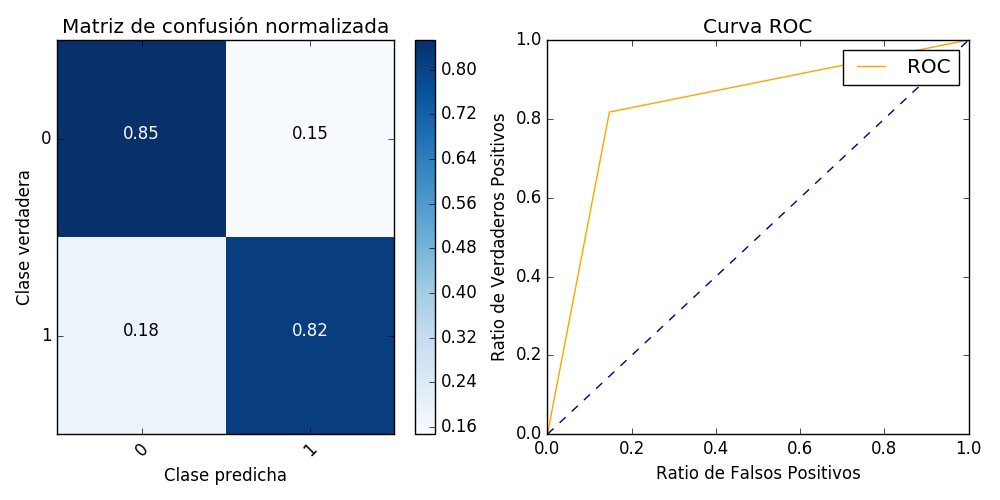
\includegraphics[width=1.0\textwidth]{TFM/figs/gra_cli_lr.png}}
\caption{Logistic Regression}
\label{fig:gra_cli_lr}
\end{figure}
Métricas:
\begin{verbatim}
Exactitud (ACC): 0.84
Error de clasificación (ERR): 0.16
Tasa de verdaderos positivos o sensibilidad (TPR | REC): 0.82
Tasa de verdaderos negativos (FPR): 0.15
Precisión (PRE)): 0.85
Especificidad(SPE): 0.85
F1: 0.83
Área bajo la curva ROC: 0.91
\end{verbatim}
%\end{minipage}

\begin{minipage}{\linewidth}
    \item Decision Tree Classifier

El Decision Tree Classifier ha obtenido uno de los peores resultados en comparación con el resto de modelos, porque ha fallado sobretodo en la tasa de verdaderos negativos (PFR).
\\

Gráficos:
\begin{figure}[H]
\centerline{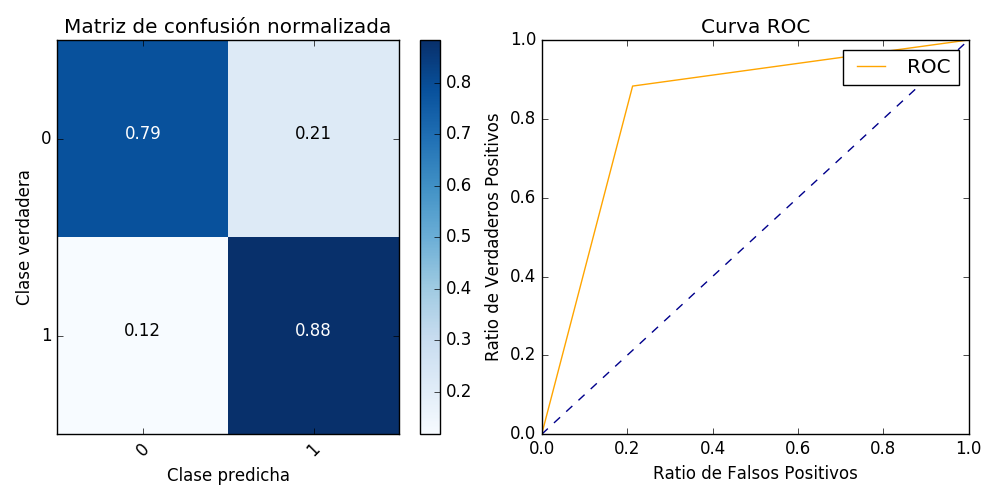
\includegraphics[width=1.0\textwidth]{TFM/figs/gra_cli_dtc.png}}
\caption{Decision Tree Classifier}
\label{fig:gra_cli_dtc}
\end{figure}
Métricas:
\begin{verbatim}
Exactitud (ACC): 0.84
Error de clasificación (ERR): 0.16
Tasa de verdaderos positivos o sensibilidad (TPR | REC): 0.88
Tasa de verdaderos negativos (FPR): 0.21
Precisión (PRE)): 0.81
Especificidad(SPE): 0.79
F1: 0.84
Área bajo la curva ROC: 0.90
\end{verbatim}
\end{minipage}

\begin{minipage}{\linewidth}
    \item Random Forest Classifier
    
El Random Forest Classifier vemos que ha fallado en lo mismo que el Decision Tree Classifier, esto puede ser explicado puesto que son de la misma familia. A continuación mostramos sus gráficos y métricas.
\\

Gráficos:
\begin{figure}[H]
\centerline{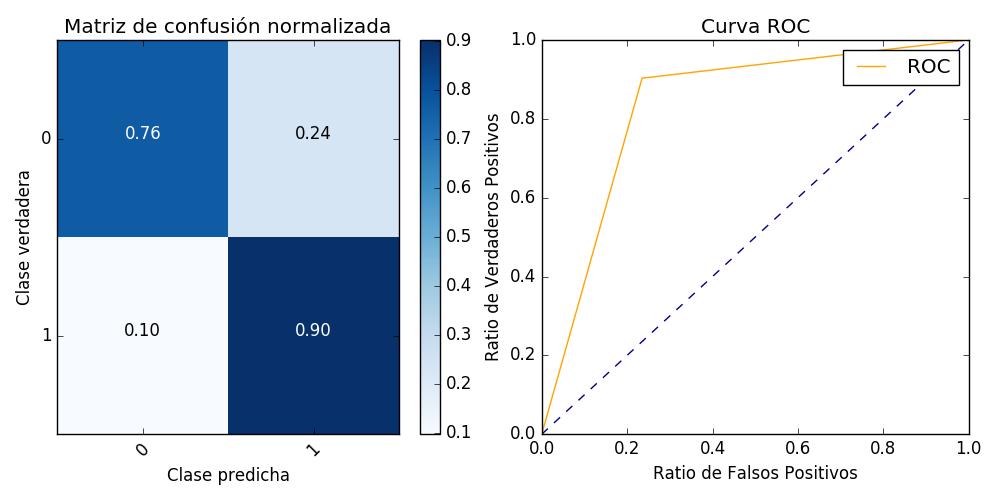
\includegraphics[width=1.0\textwidth]{TFM/figs/gra_cli_rfc.png}}
\caption{Random Forest Classifier}
\label{fig:gra_cli_rfc}
\end{figure}
Métricas:
\begin{verbatim}
Exactitud (ACC): 0.83
Error de clasificación (ERR): 0.17
Tasa de verdaderos positivos o sensibilidad (TPR | REC): 0.90
Tasa de verdaderos negativos (FPR): 0.24
Precisión (PRE): 0.79
Especificidad(SPE): 0.76
F1: 0.84
Área bajo la curva ROC: 0.91
\end{verbatim}
\end{minipage}

\begin{minipage}{\linewidth}
    \item Gradient-boosted Tree Classifier
    
El Gradient-boosted Tree Classifier ha obtenido uno de los mejores resultados, como podemos apreciar en los gráficos y métricas a continuación:
\\

Gráficos:
\begin{figure}[H]
\centerline{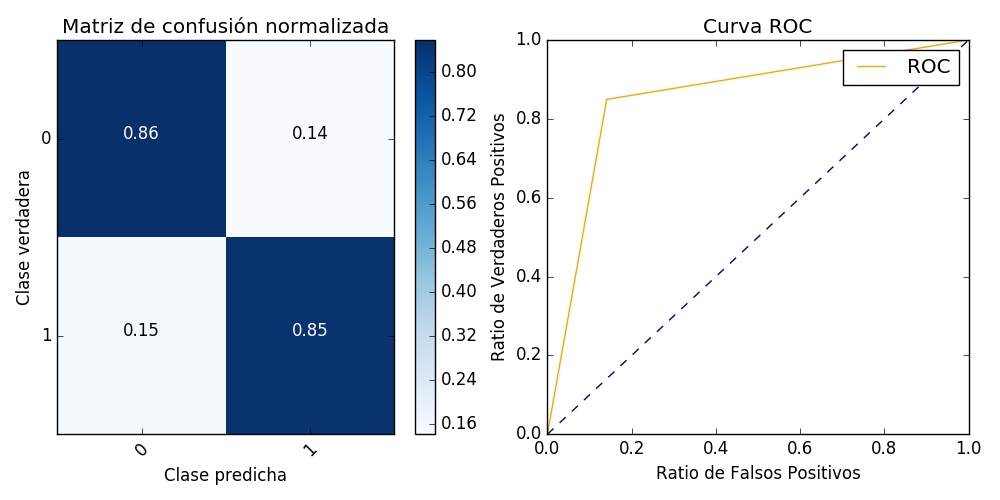
\includegraphics[width=1.0\textwidth]{TFM/figs/gra_cli_gbtc.png}}
\caption{Gradient-boosted Tree Classifier}
\label{fig:gra_cli_gbtc}
\end{figure}
Métricas:
\begin{verbatim}
Exactitud (ACC): 0.85
Error de clasificación (ERR): 0.15
Tasa de verdaderos positivos o sensibilidad (TPR | REC): 0.85
Tasa de verdaderos negativos (FPR): 0.14
Precisión (PRE): 0.86
Especificidad(SPE): 0.86
F1: 0.85
Área bajo la curva ROC: 0.93
\end{verbatim}
\end{minipage}

\begin{minipage}{\linewidth}
    \item Linear Support Vector Machine

Este modelo ha sido el que mejor calidad muestra en el objetivo de la predicción de facturación electrónica.
Como se puede observar a continuación, este modelo obtiene las mejores métricas de entre todos los modelos.
\\

Gráficos:
\begin{figure}[H]
\centerline{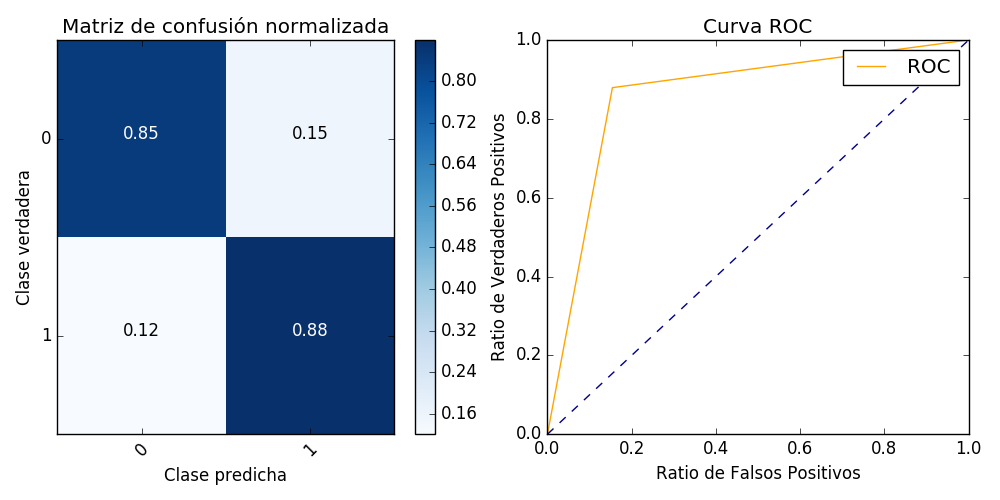
\includegraphics[width=1.0\textwidth]{TFM/figs/gra_cli_lsvm.png}}
\caption{Linear Support Vector Machine}
\label{fig:gra_cli_lsvm}
\end{figure}
Métricas:
\begin{verbatim}
Exactitud (ACC): 0.86
Error de clasificación (ERR): 0.14
Tasa de verdaderos positivos o sensibilidad (TPR | REC): 0.88
Tasa de verdaderos negativos (FPR): 0.15
Precisión (PRE)): 0.85
Especificidad(SPE): 0.85
F1: 0.86
Área bajo la curva ROC: 0.93
\end{verbatim}
\end{minipage}

\end{itemize}
\clearpage

\subsection{Predicción del canal por el que se ha realizado una reclamación}
Como veremos a continuación, los modelos de predicción del canal por el que se ha realizado una reclamación no han obtenido tan buenos resultados como los del anterior objetivo. Estos modelos han obtenido una exactitud y F1 en torno al 0.8.

\begin{itemize}

\begin{minipage}{\linewidth}
    \item Logistic Regression
    
El modelo de Logistic Regression ha obtenido una baja calidad en comparación con el resto de modelos para este objetivo, siendo su exactitud y F1 en torno a 0.75.
\\

Gráficos:    
\begin{figure}[H]
\centerline{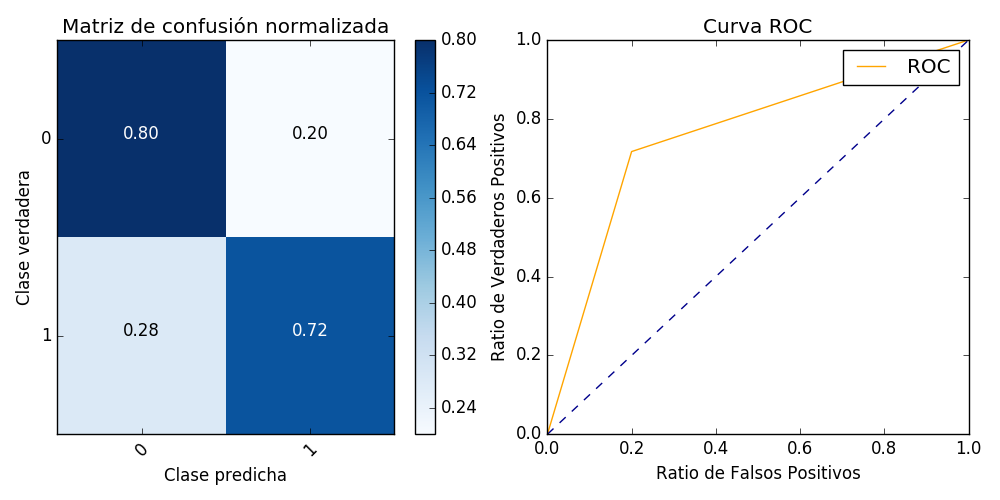
\includegraphics[width=1.0\textwidth]{TFM/figs/gra_acc_lr.png}}
\caption{Logistic Regression}
\label{fig:gra_acc_lr}
\end{figure}
Métricas:
\begin{verbatim}
Exactitud (ACC): 0.76
Error de clasificación (ERR): 0.24
Tasa de verdaderos positivos o sensibilidad (TPR | REC): 0.72
Tasa de verdaderos negativos (FPR): 0.20
Precisión (PRE)): 0.78
Especificidad(SPE): 0.80
F1: 0.75
Área bajo la curva ROC: 0.84
\end{verbatim}
\end{minipage}

\begin{minipage}{\linewidth}
    \item Decision Tree Classifier
    
El modelo Decision Tree Classifier ha obtenido uno de los mejores resultados, siendo su exactitud/F1 en torno al 0.8.
\\

Gráficos:
\begin{figure}[H]
\centerline{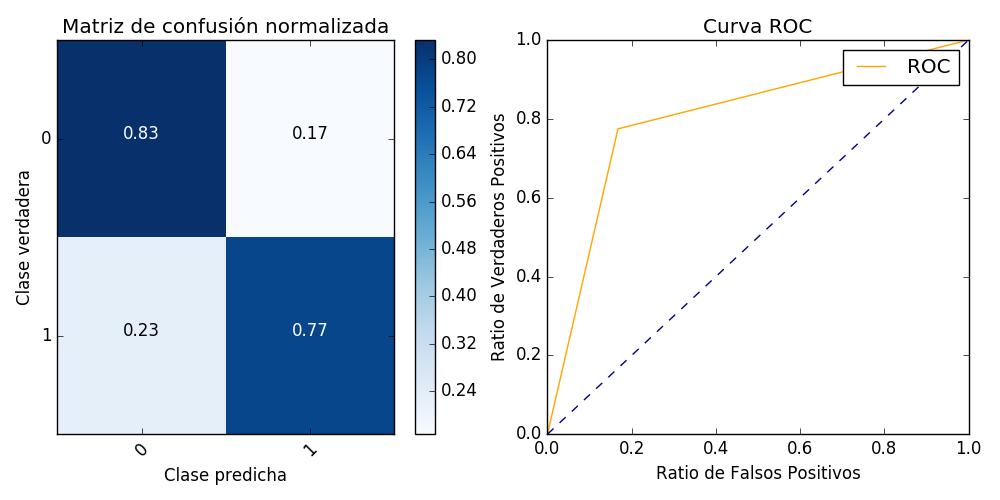
\includegraphics[width=1.0\textwidth]{TFM/figs/gra_acc_dtc.png}}
\caption{Decision Tree Classifier}
\label{fig:gra_acc_dtc}
\end{figure}
Métricas:
\begin{verbatim}
Exactitud (ACC): 0.80
Error de clasificación (ERR): 0.20
Tasa de verdaderos positivos o sensibilidad (TPR | REC): 0.77
Tasa de verdaderos negativos (FPR): 0.17
Precisión (PRE)): 0.82
Especificidad(SPE): 0.83
F1: 0.80
Área bajo la curva ROC: 0.82
\end{verbatim}
\end{minipage}

\begin{minipage}{\linewidth}
    \item Random Forest Classifier
    
El modelo Random Forest Classifier ha obtenido una buena calidad aunque un poco menor que su homólogo Decision Tree Classifier.
\\

Gráficos:
\begin{figure}[H]
\centerline{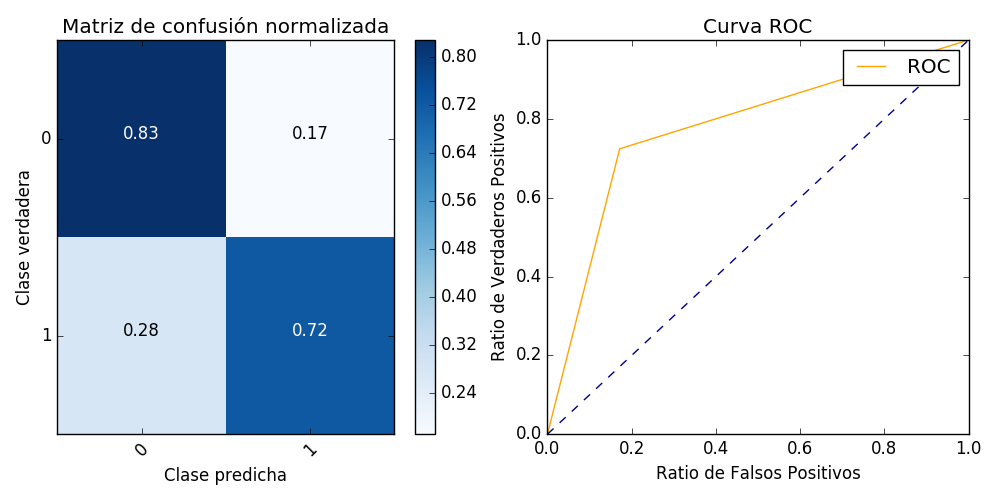
\includegraphics[width=1.0\textwidth]{TFM/figs/gra_acc_rfc.png}}
\caption{Random Forest Classifier}
\label{fig:gra_acc_rfc}
\end{figure}
Métricas:
\begin{verbatim}
Exactitud (ACC): 0.78
Error de clasificación (ERR): 0.22
Tasa de verdaderos positivos o sensibilidad (TPR | REC): 0.72
Tasa de verdaderos negativos (FPR): 0.17
Precisión (PRE)): 0.81
Especificidad(SPE): 0.83
F1: 0.76
Área bajo la curva ROC: 0.85
\end{verbatim}
\end{minipage}

\begin{minipage}{\linewidth}
    \item Gradient-boosted Tree Classifier
    
Este modelo ha sido el que mejores resultados ha conseguido en la predicción de este objetivo, siendo su exactitud/F1 de un 0.8 aproximadamente.
\\

Gráficos:
\begin{figure}[H]
\centerline{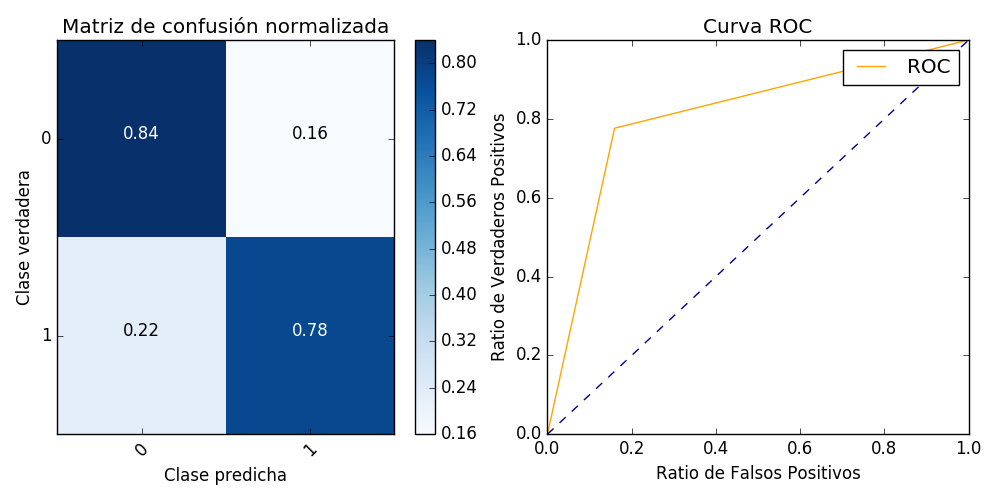
\includegraphics[width=1.0\textwidth]{TFM/figs/gra_acc_gbtc.png}}
\caption{Gradient-boosted Tree Classifier}
\label{fig:gra_acc_gbtc}
\end{figure}
Métricas:
\begin{verbatim}
Exactitud (ACC): 0.81
Error de clasificación (ERR): 0.19
Tasa de verdaderos positivos o sensibilidad (TPR | REC): 0.78
Tasa de verdaderos negativos (FPR): 0.16
Precisión (PRE)): 0.83
Especificidad(SPE): 0.84
F1: 0.80
Área bajo la curva ROC: 0.89
\end{verbatim}
\end{minipage}

\begin{minipage}{\linewidth}
    \item Linear Support Vector Machine
    
El modelo Linear Support Vector Machine ha obtenido una baja calidad en comparación a otros modelos en este mismo objetivo. 
\\

Gráficos:
\begin{figure}[H]
\centerline{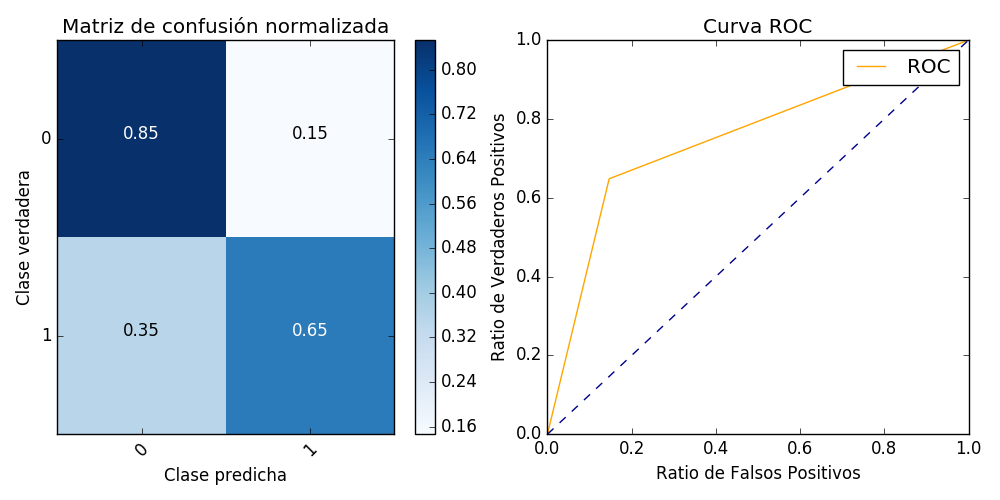
\includegraphics[width=1.0\textwidth]{TFM/figs/gra_acc_lsvm.png}}
\caption{Linear Support Vector Machine}
\label{fig:gra_acc_lsvm}
\end{figure}
Métricas:
\begin{verbatim}
Exactitud (ACC): 0.75
Error de clasificación (ERR): 0.25
Tasa de verdaderos positivos o sensibilidad (TPR | REC): 0.65
Tasa de verdaderos negativos (FPR): 0.15
Precisión (PRE)): 0.82
Especificidad(SPE): 0.85
F1: 0.72
Área bajo la curva ROC: 0.82
\end{verbatim}
\end{minipage}

\end{itemize}


\chapter{Conclusiones}
\label{chapter:conclusiones}

Mi valoración, en general, ha sido muy positiva porque hemos trabajado en el ciclo completo de un proyecto analítico de \textit{``Big Data"} con datos reales de mi actual empresa, y hemos conseguido desarrollar los objetivos parciales planteados en el inicio del proyecto. Así pues, se han realizado dos análisis predictivos clasificatorios distintos:
\begin{itemize}
    \item Predicción de facturación electrónica de los clientes.
    \item Predicción del canal por el que se ha realizado una reclamación.
\end{itemize}

Cabe recalcar que, puesto que el proyecto pertenece al aula \textit{``Big Data Analytics"}, hemos usado únicamente entornos de este tipo para su consecución.
A pesar de encontrarnos con un entorno Azure HDInsight todavía con carencias por estar en una fase temprana de despliegue, hemos podido continuar con el desarrollo en el entorno Databricks Community Edition. Como ambos sistemas son compatibles por usar Apache Spark, cuando estos errores detectados se solventen se podrán migrar todos los modelos sin mayor problema.

\\

Además, la realización del TFM me ha ayudado a profundizar conocimientos vistos en otras asignaturas del máster, así como a adquirir y aprender nuevas habilidades y tecnologías.
Algunas de las materias trabajadas han:
\begin{itemize}
    \item Profundiar el conocimiento del lenguaje de programación Python.
    \item Ampliar el conocimiento en el uso de librerías de \textit{``Machine Learning"} como Apache MLlib \cite{mllib}.
    \item Trabajar con una metodología \textit{``Agile"}.
    \item Aprender el lenguaje LaTeX\cite{latex} para la redacción de la memoria.
\end{itemize}
\\


\chapter{Líneas de trabajo futuras}
\label{chapter:lineasdetrabajo}

La realización de este TFM ha abierto nuevas posibilidades de investigación o lineas de trabajo:
\begin{itemize}
    \item Desarrollar más modelos predictivos de clasificación para otras clases, de forma que amplíen información sobre el campo estudiado.
    \item Utilizar otros modelos de \textit{``Machine Learning"}, como redes neuronales.
    \item Desplegar por completo el proceso en el entorno \textit{``Big Data"} Azure HDInsight disponible en la empresa.
\end{itemize}






% bibliografia
\addcontentsline{toc}{chapter}{Bibliografía}
\bibliographystyle{plain}
\bibliography{referencias}


\end{document}